% ==============================================================================
% ĐỀ ÔN TẬP TOÁN 6 - GIỮA HỌC KÌ I (2026 - 2027)
% 100% Nội dung từ file "Ôn tập Toán 6 GKI (26-27).docx"
% Không có phần tự luận - Bỏ tiêu đề lớn trường/lớp - Tất cả hình vẽ dùng TikZ
% ==============================================================================

\begin{center}
	{\Large\bfseries ÔN TẬP TOÁN 6 GIỮA HỌC KÌ I}\\[4pt]
	\textbf{NĂM HỌC 2026 -- 2027}
\end{center}

\vspace{6pt}

% ------------------------------------------------------------------------------
% PHẦN I: TRẮC NGHIỆM NHIỀU PHƯƠNG ÁN LỰA CHỌN
% ------------------------------------------------------------------------------
\noindent\textbf{PHẦN I. Câu trắc nghiệm nhiều phương án lựa chọn.}\\
\textit{Thí sinh trả lời từ câu 1 đến câu 20. Mỗi câu hỏi thí sinh chỉ chọn một phương án.}

\setcounter{ex}{0}

\begin{ex}%Câu 1
	Tìm cách viết đúng trong các cách viết sau?
	\choice
	{$\dfrac{4}{5} \in \mathbb{N}$}
	{$0 \in \mathbb{N}^*$}
	{\True $0 \in \mathbb{N}$}
	{$0 \notin \mathbb{N}$}
	\loigiai{
		Số $0$ là một số tự nhiên nên cách viết đúng là $0 \in \mathbb{N}$. Chọn C.
	}
\end{ex}

\begin{ex}%Câu 2
	Chữ số $5$ trong số $3\,859$ có giá trị là:
	\choice
	{$5$}
	{\True $50$}
	{$500$}
	{$5\,000$}
	\loigiai{
		Chữ số $5$ nằm ở hàng chục nên có giá trị là $50$. Chọn B.
	}
\end{ex}

\begin{ex}%Câu 3
	Cho tập hợp $A = \{0; 1; 3; 8; 9\}$, khẳng định nào sau đây là đúng?
	\choice
	{$2 \in A$}
	{$4 \in A$}
	{$5 \notin A$}
	{\True $3 \in A$}
	\loigiai{
		Phần tử $3$ thuộc tập hợp $A$ nên khẳng định đúng là $3 \in A$. Chọn D.
	}
\end{ex}

\begin{ex}%Câu 4
	Lũy thừa với số mũ tự nhiên có tính chất nào sau đây?
	\choice
	{$a^m \cdot a^n = a^{m \cdot n}$}
	{\True $a^m \cdot a^n = a^{m+n}$}
	{$a^m \cdot a^n = a^{m-n}$}
	{$a^m : a^n = a^{m:n}$}
	\loigiai{
		Khi nhân hai lũy thừa cùng cơ số, ta giữ nguyên cơ số và cộng các số mũ: $a^m \cdot a^n = a^{m+n}$. Chọn B.
	}
\end{ex}

\begin{ex}%Câu 5
	Số nào sau đây chia hết cho $2$ nhưng không chia hết cho $5$?
	\choice
	{$140$}
	{\True $146$}
	{$145$}
	{$210$}
	\loigiai{
		Số $146$ có chữ số tận cùng là $6$ nên chia hết cho $2$ nhưng không chia hết cho $5$. Chọn B.
	}
\end{ex}

\begin{ex}%Câu 6
	Trong các số: $2; 8; 16; 28$, số nào là số nguyên tố?
	\choice
	{\True $2$}
	{$8$}
	{$16$}
	{$28$}
	\loigiai{
		Số $2$ chỉ có hai ước là $1$ và $2$ nên $2$ là số nguyên tố. Các số $8; 16; 28$ là hợp số. Chọn A.
	}
\end{ex}

\begin{ex}%Câu 7
	Lũy thừa với số mũ tự nhiên có tính chất nào sau đây?
	\choice
	{$a^m : a^n = a^{m \cdot n}$}
	{$a^m : a^n = a^{m+n}$}
	{\True $a^m : a^n = a^{m-n}$ ($a \neq 0, m \ge n$)}
	{$a^m : a^n = a^{m:n}$}
	\loigiai{
		Khi chia hai lũy thừa cùng cơ số (khác $0$), ta giữ nguyên cơ số và trừ các số mũ: $a^m : a^n = a^{m-n}$ ($a \neq 0, m \ge n$). Chọn C.
	}
\end{ex}

\begin{ex}%Câu 8
	Cho hình thang cân $ABCD$ như hình vẽ. Khẳng định nào sau đây là sai?
	\begin{center}\vspace{-4pt}
		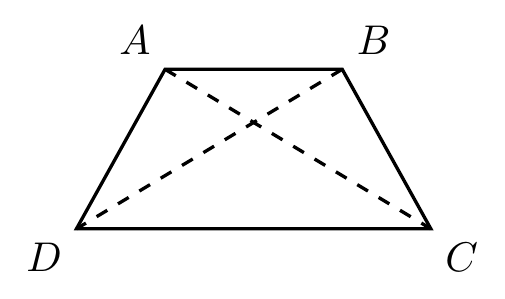
\includegraphics[height=2.2cm]{images_deontap/cau8.png}\vspace{-4pt}
	\end{center}
	\choice[2]
	{Hai cạnh đáy $AB$ và $CD$ song song với nhau}
	{Hai cạnh bên $AD$ và $BC$ bằng nhau}
	{Hai đường chéo $AC$ và $BD$ bằng nhau}
	{\True Hai đường chéo $AC$ và $BD$ vuông góc với nhau}
	\loigiai{
		Trong hình thang cân, hai đáy song song, hai cạnh bên bằng nhau, hai đường chéo bằng nhau. Hai đường chéo không nhất thiết vuông góc với nhau, do đó khẳng định sai là D.
	}
\end{ex}

\begin{ex}%Câu 9
	Tập hợp số tự nhiên khác $0$ được kí hiệu là
	\choice
	{$\mathbb{N} = \{0; 1; 2; 3; \dots\}$}
	{\True $\mathbb{N}^* = \{1; 2; 3; \dots\}$}
	{$\mathbb{N} = \{1; 2; 3; \dots\}$}
	{$\mathbb{N}^* = \{0; 1; 2; 3; \dots\}$}
	\loigiai{
		Tập hợp các số tự nhiên khác $0$ được kí hiệu là $\mathbb{N}^* = \{1; 2; 3; \dots\}$. Chọn B.
	}
\end{ex}

\begin{ex}%Câu 10
	Tập hợp các bội nhỏ hơn $20$ của $6$ là:
	\choice
	{$\{0; 6; 12; 18; \dots\}$}
	{$\{6; 12; 18\}$}
	{\True $\{0; 6; 12; 18\}$}
	{$\{1; 2; 3; 6\}$}
	\loigiai{
		Các bội của $6$ là: $0; 6; 12; 18; 24; \dots$ Do đó các bội nhỏ hơn $20$ của $6$ là $\{0; 6; 12; 18\}$. Chọn C.
	}
\end{ex}

\begin{ex}%Câu 11
	Tập hợp các chữ cái trong cụm từ TÂY NINH là:
	\choice
	{$\{\text{TÂY}; \text{NINH}\}$}
	{$\{\text{T}; \text{Â}; \text{Y}; \text{N}; \text{I}; \text{N}; \text{H}\}$}
	{$\{\text{T}; \text{A}; \text{Y}; \text{N}; \text{I}; \text{N}; \text{H}\}$}
	{\True $\{\text{T}; \text{Â}; \text{Y}; \text{N}; \text{I}; \text{H}\}$}
	\loigiai{
		Trong một tập hợp, mỗi phần tử chỉ được liệt kê một lần. Chữ N xuất hiện 2 lần nên chỉ viết 1 lần. Tập hợp các chữ cái là $\{\text{T}; \text{Â}; \text{Y}; \text{N}; \text{I}; \text{H}\}$. Chọn D.
	}
\end{ex}

\begin{ex}%Câu 12
	Đối với các biểu thức có dấu ngoặc, thứ tự thực hiện phép tính là
	\choice
	{$[\ ] \to (\ ) \to \{\ \}$}
	{\True $(\ ) \to [\ ] \to \{\ \}$}
	{$\{\ \} \to (\ ) \to [\ ]$}
	{$\{\ \} \to [\ ] \to (\ )$}
	\loigiai{
		Thứ tự thực hiện phép tính có ngoặc là: $(\ ) \to [\ ] \to \{\ \}$. Chọn B.
	}
\end{ex}

\begin{ex}%Câu 13
	Trong các số sau, số nào là hợp số?
	\choice
	{$5$}
	{\True $18$}
	{$7$}
	{$3$}
	\loigiai{
		Số $18$ có nhiều hơn hai ước ($1; 2; 3; 6; 9; 18$) nên $18$ là hợp số. Chọn B.
	}
\end{ex}

\begin{ex}%Câu 14
	Số nào trong các số sau đây chia hết cho $3$ mà không chia hết cho $9$?
	\choice
	{\True $2\,019$}
	{$288$}
	{$999$}
	{$36$}
	\loigiai{
		Số $2\,019$ có tổng các chữ số là $2 + 0 + 1 + 9 = 12$, chia hết cho $3$ nhưng không chia hết cho $9$. Chọn A.
	}
\end{ex}

\begin{ex}%Câu 15
	Cho tập hợp $A = \{1; 6; 7; 9\}$, khẳng định nào sau đây là đúng?
	\choice
	{$2 \in A$}
	{\True $6 \in A$}
	{$9 \notin A$}
	{$3 \in A$}
	\loigiai{
		Phần tử $6$ thuộc tập hợp $A$ nên khẳng định đúng là $6 \in A$. Chọn B.
	}
\end{ex}

\begin{ex}%Câu 16
	Khẳng định nào dưới đây là đúng? Trong hình bình hành:
	\choice[2]
	{Bốn góc bằng nhau}
	{Hai đường chéo bằng nhau}
	{Bốn cạnh bằng nhau}
	{\True Hai đường chéo cắt nhau tại trung điểm mỗi đường}
	\loigiai{
		Trong hình bình hành, hai đường chéo cắt nhau tại trung điểm của mỗi đường. Chọn D.
	}
\end{ex}

\begin{ex}%Câu 17
	Tập hợp các bội nhỏ hơn $30$ của $7$ là:
	\choice
	{$\{0; 7; 14; 21; 28; \dots\}$}
	{$\{7; 14; 21; 28\}$}
	{\True $\{0; 7; 14; 21; 28\}$}
	{$\{1; 7\}$}
	\loigiai{
		Các bội của $7$ nhỏ hơn $30$ là: $0; 7; 14; 21; 28$. Chọn C.
	}
\end{ex}

\begin{ex}%Câu 18
	Số nào sau đây chia hết cho $3$ nhưng không chia hết cho $9$?
	\choice
	{\True $120$}
	{$1\,035$}
	{$1\,475$}
	{$108$}
	\loigiai{
		Số $120$ có tổng các chữ số là $1 + 2 + 0 = 3$, chia hết cho $3$ nhưng không chia hết cho $9$. Chọn A.
	}
\end{ex}

\begin{ex}%Câu 19
	Trong các số: $0; 7; 22; 36$, số nào là số nguyên tố?
	\choice
	{$0$}
	{\True $7$}
	{$22$}
	{$36$}
	\loigiai{
		Số $7$ chỉ có hai ước tự nhiên là $1$ và $7$ nên $7$ là số nguyên tố. Chọn B.
	}
\end{ex}

\begin{ex}%Câu 20
	Số nào sau đây chia hết cho cả $2$ và $5$?
	\choice
	{$1\,235$}
	{\True $1\,230$}
	{$1\,232$}
	{$2\,025$}
	\loigiai{
		Số chia hết cho cả $2$ và $5$ có chữ số tận cùng bằng $0$, do đó chọn $1\,230$.
	}
\end{ex}
\vspace{2pt}

% ------------------------------------------------------------------------------
% PHẦN II: CÂU TRẮC NGHIỆM ĐÚNG SAI
% ------------------------------------------------------------------------------
\noindent\textbf{PHẦN II. Câu trắc nghiệm đúng sai.}\\
\textit{Thí sinh trả lời từ câu 21 đến câu 25. Trong mỗi ý a), b), c), d) ở mỗi câu, thí sinh chọn đúng hoặc sai.}

\begin{ex}%Câu 21
	Xét tính đúng/sai của các khẳng định sau về tam giác đều:
	\choiceTF
	{\True Ba góc bằng nhau và mỗi góc bằng $60^\circ$}
	{Tam giác đều có ba cạnh bằng nhau và ba góc khác nhau}
	{Tam giác đều có một góc vuông}
	{\True Tất cả các cạnh của tam giác đều bằng nhau}
	\loigiai{
		\begin{itemchoice}
			\item Đúng: Tam giác đều có ba góc bằng nhau và mỗi góc bằng $60^\circ$.
			\item Sai: Tam giác đều có ba góc bằng nhau chứ không khác nhau.
			\item Sai: Tam giác đều không có góc vuông (mỗi góc bằng $60^\circ$).
			\item Đúng: Tất cả ba cạnh của tam giác đều bằng nhau.
		\end{itemchoice}
	}
\end{ex}

\begin{ex}%Câu 22
	Xét tính đúng/sai của các khẳng định sau về hình bình hành:
	\choiceTF
	{Hình bình hành có bốn cạnh bằng nhau}
	{\True Hình bình hành có các cạnh đối bằng nhau}
	{Hình bình hành có hai đường chéo bằng nhau}
	{Hình bình hành có các góc đều bằng nhau}
	\loigiai{
		\begin{itemchoice}
			\item Sai: Hình bình hành có các cạnh đối bằng nhau, không bắt buộc bốn cạnh bằng nhau.
			\item Đúng: Trong hình bình hành, các cạnh đối song song và bằng nhau.
			\item Sai: Hai đường chéo của hình bình hành không nhất thiết bằng nhau.
			\item Sai: Trong hình bình hành, chỉ có các góc đối bằng nhau.
		\end{itemchoice}
	}
\end{ex}

\begin{ex}%Câu 23
	Xét tính đúng/sai của các khẳng định sau về hình thoi:
	\choiceTF
	{Các cặp cạnh đối của hình thoi không bằng nhau và song song}
	{Hai đường chéo của hình thoi cắt nhau tại trung điểm của mỗi đường}
	{\True Các góc đối nhau bằng nhau}
	{\True Hình thoi có bốn cạnh bằng nhau}
	\loigiai{
		\begin{itemchoice}
			\item Sai: Các cặp cạnh đối diện của hình thoi bằng nhau và song song.
			\item Sai (theo bảng đáp án của đề): Trong đề thi, ý này được xếp loại Sai. \textit{Mở rộng:} Hình thoi là trường hợp đặc biệt của hình bình hành nên hai đường chéo cắt nhau tại trung điểm mỗi đường và vuông góc với nhau.
			\item Đúng: Các góc đối diện trong hình thoi bằng nhau.
			\item Đúng: Hình thoi có bốn cạnh bằng nhau.
		\end{itemchoice}
	}
\end{ex}

\begin{ex}%Câu 24
	Xét tính đúng/sai của các khẳng định sau về hình bình hành:
	\choiceTF
	{\True Hai đường chéo của hình bình hành cắt nhau tại trung điểm mỗi đường}
	{Các góc đối trong hình bình hành không bằng nhau}
	{Hình bình hành có bốn cạnh bằng nhau}
	{\True Hình bình hành có các cạnh đối bằng nhau}
	\loigiai{
		\begin{itemchoice}
			\item Đúng: Hai đường chéo của hình bình hành cắt nhau tại trung điểm của mỗi đường.
			\item Sai: Các góc đối diện trong hình bình hành bằng nhau.
			\item Sai: Hình bình hành có các cạnh đối bằng nhau, không nhất thiết bốn cạnh bằng nhau.
			\item Đúng: Các cạnh đối diện của hình bình hành bằng nhau.
		\end{itemchoice}
	}
\end{ex}

\begin{ex}%Câu 25
	Xét tính đúng/sai của các khẳng định sau về hình thoi và hình thang cân:
	\choiceTF
	{\True Hình thoi có $4$ cạnh bằng nhau và các cạnh đối song song}
	{Hai đường chéo của hình thoi bằng nhau}
	{\True Hình thang cân có hai cạnh bên bằng nhau và hai góc kề một đáy bằng nhau}
	{Hai đường chéo của hình thang cân luôn vuông góc với nhau}
	\loigiai{
		\begin{itemchoice}
			\item Đúng: Hình thoi có $4$ cạnh bằng nhau và các cặp cạnh đối song song.
			\item Sai: Hai đường chéo của hình thoi vuông góc với nhau nhưng thường có độ dài khác nhau.
			\item Đúng: Hình thang cân có hai cạnh bên bằng nhau và hai góc kề một đáy bằng nhau.
			\item Sai: Hai đường chéo của hình thang cân bằng nhau nhưng không nhất thiết vuông góc với nhau.
		\end{itemchoice}
	}
\end{ex}

\newpage

% ------------------------------------------------------------------------------
% PHẦN III: CÂU TRẮC NGHIỆM TRẢ LỜI NGẮN
% ------------------------------------------------------------------------------
\noindent\textbf{PHẦN III. Câu trắc nghiệm trả lời ngắn.}\\
\textit{Thí sinh trả lời từ câu 26 đến câu 35.}

\begin{ex}%Câu 26
	Tìm các bội nhỏ hơn $40$ của $6$?
	\shortans{0; 6; 12; 18; 24; 30; 36}
	\loigiai{
		Các bội của $6$ nhỏ hơn $40$ là: $\{0; 6; 12; 18; 24; 30; 36\}$.
	}
\end{ex}

\begin{ex}%Câu 27
	Viết số La Mã $\mathrm{XXIV}, \mathrm{XXVI}, \mathrm{XIX}, \mathrm{XIV}$ sang số tự nhiên trong hệ thập phân.
	\shortans{24; 26; 19; 14}
	\loigiai{
		Ta có:
		\begin{itemize}
			\item $\mathrm{XXIV} = 10 + 10 + 4 = 24$.
			\item $\mathrm{XXVI} = 10 + 10 + 6 = 26$.
			\item $\mathrm{XIX} = 10 + 9 = 19$.
			\item $\mathrm{XIV} = 10 + 4 = 14$.
		\end{itemize}
		Các số tự nhiên tương ứng là: $24; 26; 19; 14$.
	}
\end{ex}

\begin{ex}%Câu 28
	Cho hình thoi $ABCD$ có độ dài cạnh $AB$ bằng $6\text{ cm}$. Tính $BC$?
	\shortans{6\text{ cm}}
	\loigiai{
		Vì hình thoi có bốn cạnh bằng nhau nên $BC = AB = 6\text{ cm}$.
	}
\end{ex}

\begin{ex}%Câu 29
	Tính diện tích mảnh ruộng hình thang có các kích thước như hình vẽ dưới đây:
	\begin{center}\vspace{-4pt}
		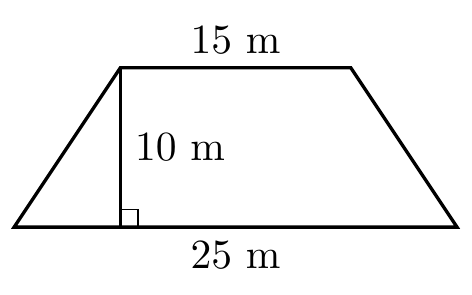
\includegraphics[height=2.2cm]{images_deontap/cau28.png}\vspace{-4pt}
	\end{center}
	\shortans{200\text{ m}^2}
	\loigiai{
		Diện tích mảnh ruộng hình thang là:
		\[ S = \frac{(15 + 25) \cdot 10}{2} = 200\text{ (m}^2\text{)}. \]
	}
\end{ex}

\begin{ex}%Câu 30
	Chữ số La Mã biểu diễn số $19, 26, 29, 15$ là:
	\shortans{XIX, XXVI, XXIX, XV}
	\loigiai{
		Biểu diễn các số dưới dạng chữ số La Mã:
		\begin{itemize}
			\item $19 \to \mathrm{XIX}$.
			\item $26 \to \mathrm{XXVI}$.
			\item $29 \to \mathrm{XXIX}$.
			\item $15 \to \mathrm{XV}$.
		\end{itemize}
		Vậy các số La Mã là: $\mathrm{XIX}, \mathrm{XXVI}, \mathrm{XXIX}, \mathrm{XV}$.
	}
\end{ex}

\begin{ex}%Câu 31
	Kết quả của phép tính $12^7 : 12^5$ bằng:
	\shortans{12^2}
	\loigiai{
		$12^7 : 12^5 = 12^{7-5} = 12^2 = 144$.
	}
\end{ex}

\begin{ex}%Câu 32
	Tính diện tích hình vuông có độ dài cạnh bằng $9\text{ cm}$.
	\shortans{81\text{ cm}^2}
	\loigiai{
		Diện tích hình vuông là:
		\[ S = 9 \cdot 9 = 81\text{ (cm}^2\text{)}. \]
	}
\end{ex}

\begin{ex}%Câu 33
	Rút gọn phân số $\dfrac{3}{6}$ đến tối giản ta được:
	\shortans{1/2}
	\loigiai{
		Chia cả tử và mẫu cho $3$, ta được phân số tối giản là $\dfrac{1}{2}$.
	}
\end{ex}

\begin{ex}%Câu 34
	Phân tích số $36$ ra thừa số nguyên tố ta được:
	\shortans{2^2 \cdot 3^2}
	\loigiai{
		Ta có: $36 = 4 \cdot 9 = 2^2 \cdot 3^2$.
	}
\end{ex}

\begin{ex}%Câu 35
	Ước chung lớn nhất của $12$ và $18$ là:
	\shortans{6}
	\loigiai{
		Ta có: $12 = 2^2 \cdot 3$ và $18 = 2 \cdot 3^2$. Suy ra $\text{ƯCLN}(12, 18) = 2 \cdot 3 = 6$.
	}
\end{ex}

